\documentclass{article}
\usepackage{graphicx}
\usepackage{url}
\usepackage{caption}
\usepackage{subcaption}

\begin{document}

\title{COMS 4107 - AI\\
Homework 3\\
Machine Learning}
\author{Matheus Cassiano Candido\\
mcc2224}

\maketitle

\section{Problem 1}

\subsection{Linear regression with one feature}
For this part, I was provided with two sets of data. The training and testing datasets, that are on files \path{girls_train.csv} and \path{girls_test.csv}, respectively. Data distribution is shown on Figure \ref{p1distribution}.

\begin{figure}[htb]
    \centering
    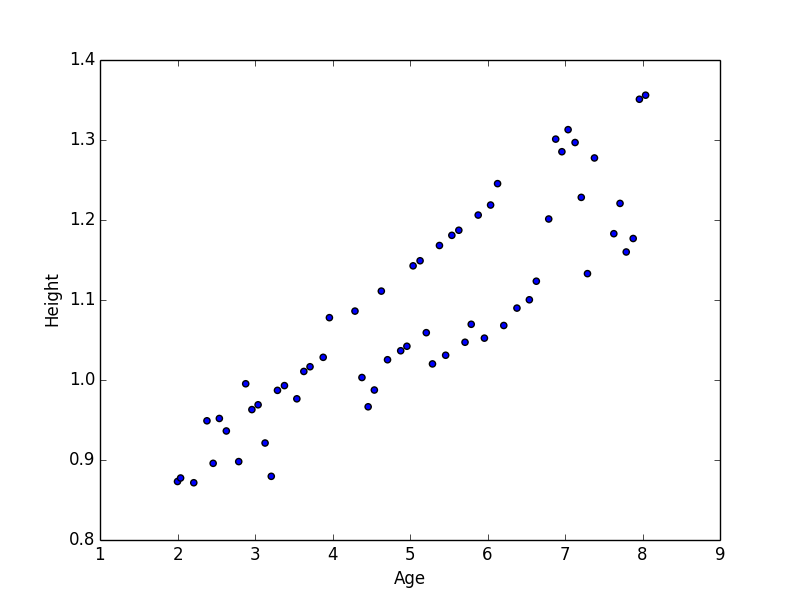
\includegraphics[width=3.0in]{p1_distribution}
    \caption{Training data distribution}
    \label{p1distribution}
\end{figure}

After implementing the Gradient Descent algorithm, I ran it on my test data using $\alpha = 0.05$ and set the number of iterations to 1500. My mean square error was of 0.001825 for the training set. My model was $0.064464x + 0.756075$ as illustrated on Figure \ref{regressionline}. The cost function has a flat bowl shape (see Figure \ref{costfunction}).

\begin{figure}[htb]
\centering
\begin{minipage}{.5\textwidth}
  \centering
  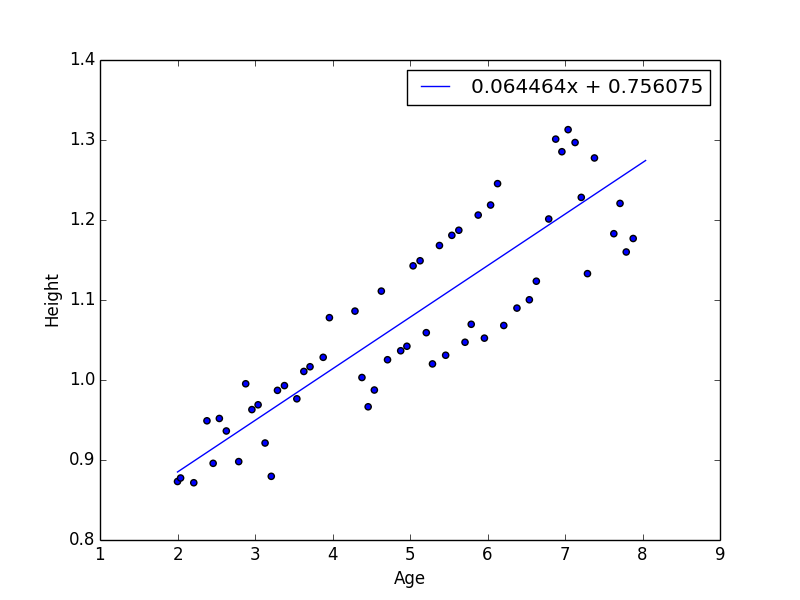
\includegraphics[width=1.0\linewidth]{regression_line}
  \captionof{figure}{Regression line}
  \label{regressionline}
\end{minipage}%
\begin{minipage}{.5\textwidth}
  \centering
  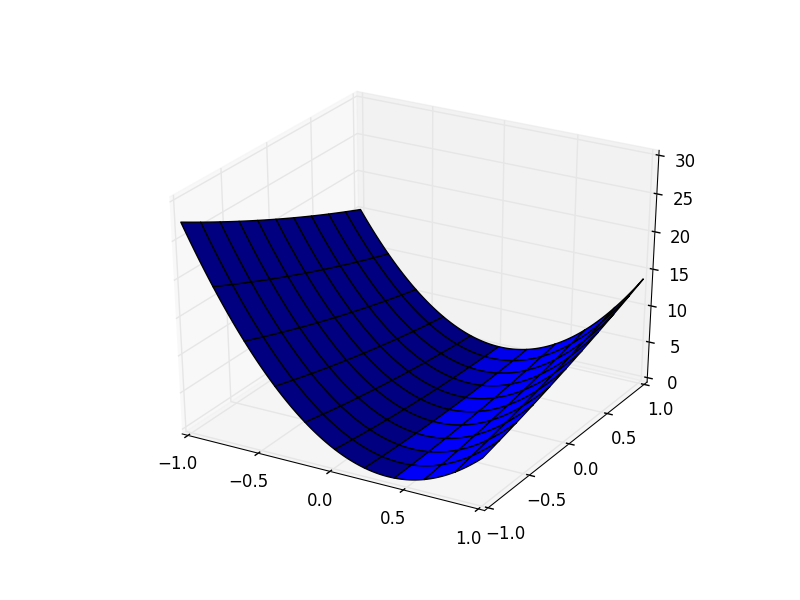
\includegraphics[width=1.0\linewidth]{p1_cost_function}
  \captionof{figure}{Cost function}
  \label{costfunction}
\end{minipage}
\end{figure}


Using my model I predicted that a 4.5 kilos girl would be approximately 1.046164 m tall, which is an accurate estimation. The model also performed well on the test set. The mean square error was 0.003203 for the 20 examples.

\subsection{Linear regression with multiple features}
The second part of this problem consisted in implementing Gradient Descent with multiple features. For this experiment, I used the \path{girls_age_weight_height_2_8.csv} dataset provided.

Before running the Gradient Descent, we were advised to scale the features. Using mean 5.210506 and standard deviaton 1.899482, I scaled the features, getting the desired $\mu(x) = 0$. The next step was choosing the best $\alpha$. I looped through all possible values (0.005, 0.001, 0.05, 0.1, 0.5, 1.0) for the learning rate using number of iterations, applying Gradient Descent for each of them.

\begin{figure}[htb]
    \centering
    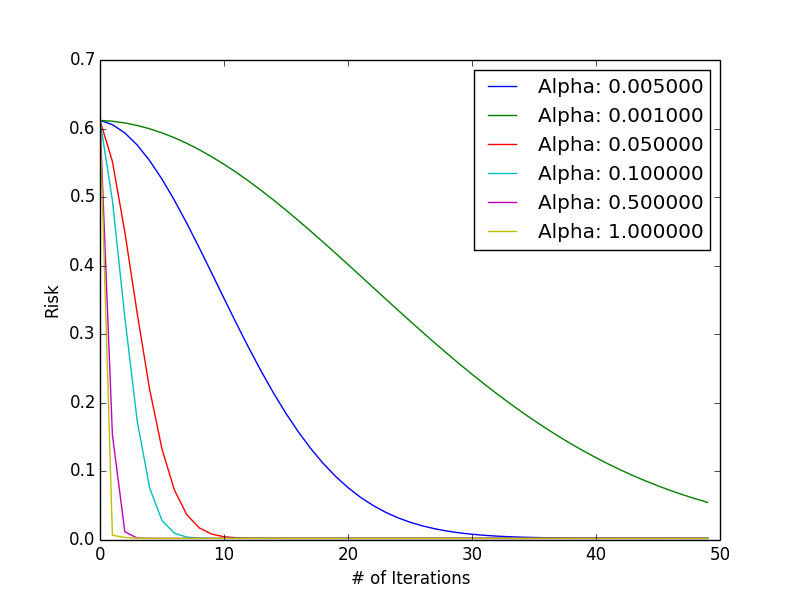
\includegraphics[width=3.0in]{p1_alpha_convergence}
    \caption{Training data distribution}
    \label{costfunction}
\end{figure}

The results for each $\alpha$ is shown on Figure \ref{costfunction}. These results show that smaller values of $\alpha$ tend to converge slower that the larger ones. The best value on this one is 1.0. The $\beta's$ are [1.09646081, 0.12861721, 0.00140248]. A predict height for a 5-year olg girl weighting 20 kilos is 1.082595 m.

\subsubsection{Linear regression with Normal Equations}
Although having the same prediction and the same error, the $\beta's$ aren't the same and that's due to the fact that when I was doing Gradient Descent with multiple variables, I scaled my dataset.

Normal Equations yield the same predictions as Gradient Descent. The reason is that both Normal Equations and Gradient Descent try to minimize the Least Squares. The thing is that NE finds a unique solution that minimizes the least squares. It is not always the best approach because its time complexity is really high. The predicted height for a 5-year olg girl weighting 20 kilos was 1.082595 m.


\section{Conclusion}
Write your conclusion here.

\end{document}